\documentclass[16pt,presentation]{beamer}
%\mode<presentation>{\usetheme{default}}
%\setbeamersize{text margin left=0.5cm} 
%\setbeamersize{text margin right=0.5cm} 

\usepackage{color}
\usepackage{rotating}
\usepackage{graphicx}
\usepackage[english]{babel}
\usepackage[latin1]{inputenc}
\usepackage{helvet}
\usepackage[T1]{fontenc}
\usepackage{units}
\usepackage{bm}
\usepackage{amssymb}
\usepackage{amsthm}
\usepackage{amsmath}
\usepackage{algorithm}
\usepackage{algorithmicx}
\usepackage{rotating}
\usepackage{hyperref}
\usepackage{tikz}
\usepackage{bbm}
\usetikzlibrary{fit,positioning}
\usepackage[backend=bibtex,style=authoryear]{biblatex}
\usepackage{pifont}% http://ctan.org/pkg/pifont
\newcommand{\cmark}{\ding{51}}%
\newcommand{\xmark}{\ding{55}}%
\addbibresource{refs.bib}

% Standard environments here
\usepackage{mathtools} % pmatrix*! use \begin{matrix*}[r] to center colums right


% ----  Custom Environments ----- 
% just a horizontal rule for the "details" environment
\newcommand{\optionrule}{\noindent\rule{1.0\textwidth}{0.75pt}}
% the "details" environment declaration.
\newenvironment{aside}{%
  \def\FrameCommand{\hspace{2em}}
  \MakeFramed {\advance\hsize-\width \small}\optionrule}
{\\\optionrule\endMakeFramed}
% I took out the newline command. i don't know what it did.
%{\newline\optionrule\endMakeFramed}

% ---- Text/Formatting Symbols ---
\renewcommand{\eqref}[1]{Equation (\ref{#1})}
\newcommand{\figref}[1]{Figure \ref{#1}}
%\renewcommand{\etal}{{\it et al} }

% ---- Math symbols ------------

% basic algebra, set-theoretic, and functional notation
\newcommand{\set}[1]{\{#1\}} % set notation
\newcommand{\Range}{\mathcal{R}} % range (ie, of a function)
\newcommand{\setcomp}[1]{{#1}^{\mathsf{c}}} % set complement
%\newcommand{\inv}{^{-1}} % inverse
\newcommand{\inv}[1]{\ensuremath{{#1}^{-1}}} 
\newcommand{\ind}[1]{\mathbf{1}_{\left\{ #1\right\}}} % indicator function
\newcommand{\sgn}{\operatorname{sgn}}

\newcommand{\st}{\mbox{ s.t. }} % such that or subject to

% number sets
% \newcommand{\N}{\mathbb N}
% \newcommand{\Z}{\mathbb Z}
% \newcommand{\Q}{\mathbb Q}
% \newcommand{\R}{\mathbb R}
% \newcommand{\C}{\mathbb C}

%\DeclareMathOperator*{\argmax}{argmax}
%\DeclareMathOperator*{\argmin}{argmin}
\DeclareMathOperator*{\supp}{supp}
\DeclareMathOperator*{\tr}{tr}

% Calculus: Derivatives \& Integrals
\newcommand{\dm}[1]{\ensuremath{\,\mathrm{d}{#1}}} % Pretty symbol for differentials - ie, dx
\newcommand{\deriv}[2]{\frac{d #1}{d #2}}
\newcommand{\D}[2]{\frac{\partial #1}{\partial #2}}
\newcommand{\DD}[2]{\frac{\partial ^2 #1}{\partial #2 ^2}}
\newcommand{\Di}[2]{\frac{\partial ^i #1}{\partial #2 ^i}}
\newcommand{\evalat}[1]{\left.#1\right|}
\newcommand{\parderiv}[2]{\frac{\partial #1}{\partial{#2}}}
\newcommand{\parDeriv}[3]{\frac{\partial^{#3} #1}{\partial{#2}^{#3}}}
\newcommand{\parwrt}[1]{\frac{\partial}{\partial{#1}}}
\newcommand{\parpowrt}[2]{\frac{\partial^{#1}}{\partial {#2}^{#1}}}
\newcommand{\partwowrt}[2]{\frac{\partial^{2}}{\partial {#2} \partial{#1}}}

% basic linear algebra notation
\newcommand{\ones}{\mathop{\mathbf{1}}} % vector of ones
\newcommand{\diag}{\mathop{\mbox{diag}}}
\newcommand{\rank}{\mathop{\mathrm{rank}}} % null space ( range is \Range, above)
\newcommand{\Null}{\mathcal N} % null space ( range is \Range, above)
\newcommand{\Tr}{\textrm{Tr}} % trace
\newcommand{\norm}[1]{\left|\left|#1\right|\right|}  % normroduct
\newcommand{\tp}[1]{\ensuremath{{#1}^\top}} % transpose with argument
\newcommand{\trp}{^{\mathrm{T}}} % Transpose
\newcommand{\itrp}{^{-\mathrm{T}}} % inverse-transpose
\newcommand{\inprod}[2]{\langle #1,#2\rangle}

% Probability notation
\newcommand{\pialg}{\pi\text{-algebra}}
\newcommand{\sigalg}{\sigma\text{-algebra}}
\newcommand{\alg}[1]{\mathcal{#1}} % sigma algebra notation
\newcommand{\E}{\mathbb{E}}
\newcommand{\V}{\mathbb{V}}
\newcommand{\Prob}[1]{\mathbb{P}\left[#1\right]}
\newcommand\independent{\protect\mathpalette{\protect\independenT}{\perp}}
\def\independenT#1#2{\mathrel{\rlap{$#1#2$}\mkern2mu{#1#2}}}
\newcommand{\Norm}[2]{\mathcal{N}\left(#1, #2\right)} % normal distribution
%\newcommand{\mvn}[4]{\frac{1}{(2\pi)^{\frac{#4}{2}} |#3|^\frac{1}{2}} 
%\exp \left[-\tfrac{1}{2} (#1 - #2)\trp #3^{-1}(#1-#2)\right]} % multivariate normal
%% Notation for specific projects
%\newcommand{\mvnzero}[2]{\frac{1}{|2\pi #2|^\frac{1}{2}}
%\exp \left[-\tfrac{1}{2} #1\trp #2^{-1}#1\right]}  % zero-mean mvn

%Yuanjun's stuff
\newcommand{\N}{\mathcal{N}}

% matrix variables
\newcommand{\identityMat}{\ensuremath{I}}

\usepackage{forloop}
\newcommand{\defvec}[1]{\expandafter\newcommand\csname v#1\endcsname{{\mathbf{#1}}}}
\newcounter{ct}
\forLoop{1}{26}{ct}{
    \edef\letter{\alph{ct}}
    \expandafter\defvec\letter
}
\newcommand{\defmat}[1]{\expandafter\newcommand\csname m#1\endcsname{{\mathbf{#1}}}}
\forLoop{1}{26}{ct}{
    \edef\letter{\Alph{ct}}
    \expandafter\defmat\letter
}
\newcommand{\vmu}{\bm{\mu}}
\newcommand{\veta}{\bm{\eta}}
\newcommand{\vepsilon}{\bm{\epsilon}}
\newcommand{\vlambda}{\bm{\lambda}}


\newcommand{\mLambda}{\bm{\Lambda}}

% mutual information symbols (for MI estimation)

% convex analysis symbols (for optimization class)
\newcommand{\conv}{\text{conv}} % convex hull
\newcommand{\aff}{\text{Aff }} % affine hull
\newcommand{\extp}{\text{Ext}} %extreme points
%\newcommand{\argmin}{\mathrm{arg}\min}
\newcommand{\argmin}[1]{\underset{#1}{\operatorname{argmin}}}
\newcommand{\argmax}[1]{\underset{#1}{\operatorname{argmax}}}
\newcommand{\grad}{\nabla}
\newcommand{\curl}{\nabla\times}
\newcommand{\logdet}[1]{\log |#1|}


%% My own TheoremStyle
  \newtheoremstyle{evandefinition}{\topsep}{\topsep}%
     {}%         Body font  (\itshape)
     {}%         Indent amount (empty = no indent, \parindent = para indent)
     {\bfseries}% Thm head font
     {}%        Punctuation after thm head
     {\newline}%  Space after thm head  (default: 5pt plus 1pt minus 1pt)
     {\thmname{#1}\thmnumber{ #2}. \textit{\thmnote{ #3} }}%         Thm head spec


     \newtheoremstyle{indenteddefinition}{\topsep}{\topsep}
     {\addtolength{\leftskip}{2em}} %         Body font  (\itshape)
     {-1.75em}%         Indent amount (empty = no indent, \parindent = para indent)
     {\bfseries}% Thm head font % also: \scshape
     {}%        Punctuation after thm head
     { }%  Space after thm head  (default: 5pt plus 1pt minus 1pt)
     {\thmname{#1} \thmnumber{#2}. \textbf{(\thmnote{#3})}}%         Thm head spec
     % {} %         Thm head spec


% %% This code will allow me to have a bar around shit (uses ntheorem)
% %\theoremstyle{plain}
% \theorembodyfont{}
% \usepackage{color}
% \definecolor{gray}{rgb}{0.7,0.7,0.7}
% % This code turns the box around the theorem into a bar to the left
% \renewcommand*\FrameCommand{{\color{gray}\vrule width 1pt\hspace{10pt}}}


% general headings
%\newtheorem{theorem}{Theorem}
%\newtheorem{lemma}{Lemma}
%\newtheorem{proposition}{Proposition}
%\newtheorem{corollary}{Corollary}

%\theoremstyle{evandefinition}
%\newtheorem{definition}{Definition}
%\theoremstyle{definition}
% \theoremindent1em
% \theorembodyfont{\normalfont}
%\newframedtheorem{definition}{Definition}

%\theoremstyle{indenteddefinition} 
%\newtheorem{example}{Example}

\theoremstyle{remark} 
\newtheorem{exercise}{Exercise}
\newtheorem{remark}{Remark}

%% Make it so matrix has an align-column option ([c])
\makeatletter
\renewcommand*\env@matrix[1][c]{\hskip -\arraycolsep
  \let\@ifnextchar\new@ifnextchar
  \array{*\c@MaxMatrixCols #1}}
\makeatother

%%%%%%%%%%%%%%%%%%%%%%%%%%%%%%%%
%% Examples of things I might want to do.
%%%%%%%%%%%%%%%%%%%%%%%%%%%%%%%%
% 
%%%%%%%%%%%%%%%%
%  Function with different cases:
%%%%%%%%%%%%%%%%
% \begin{align*}
%   q(\mu) &= \inf_x L(x,\mu)
% \\
% &=\left\{
% \begin{matrix}
% &c_0 + \mu c_1 - (b_0 - \mu b_1)^T ( A_0 + \mu A_1)^+ (b_0 + \mu
% b_1 )^T  &  A_0 + \mu A_1 \succeq 0,
% \\
% &\quad & b_0 + \mu b_1 \in \mathcal{R}(A_0 + \mu A_1)
% \\
% & \infty & \mathrm{otherwise}
% \end{matrix}\right.
% \end{align*}
% 



%TODO
% add citation


%\usetheme{Warsaw}
\usetheme{metropolis}

\setbeamerfont{footline}{size=\fontsize{6}{10}\selectfont}

%%%% title etc.
\author[Yuanjun Gao]{Yuanjun Gao}
\institute{\small Department of Statistics\\ Columbia University}
\title[Department of Statistics, Columbia University]{\large Statistical Machine Learning Methods for High-dimensional Neural Population Data Analysis}
\date{}

\begin{document}

\defbeamertemplate{subsection in toc}{bullets}{%
  \leavevmode
  \parbox[t]{2em}{\hspace{1em}\textbullet\hfill}%
  \parbox[t]{\dimexpr\textwidth-1em\relax}{\inserttocsubsection}\par}
\defbeamertemplate{section in toc}{sections numbered roman}{%
  \leavevmode%
  \MakeUppercase{\romannumeral\inserttocsectionnumber}.\ %
  \inserttocsection\par}

\beamertemplatetransparentcovereddynamicmedium
\setbeamertemplate{section in toc}[sections numbered roman]
\setbeamertemplate{subsection in toc}[bullets]
\setbeamercolor{background canvas}{bg=white}


%%%%%%%%%%%%%%%%%%% Title page %%%%%%%%%%%%%%%%%
\begin{frame}\vspace*{1.5cm}
\maketitle
\begin{center}
\vspace{-1cm}
\end{center}
\end{frame}


%%%%%%%%%%%%%%%%%%%%%%%% Overview %%%%%%%%%%%%%%%%%%
\begin{frame}
\frametitle{Overview}
\centering
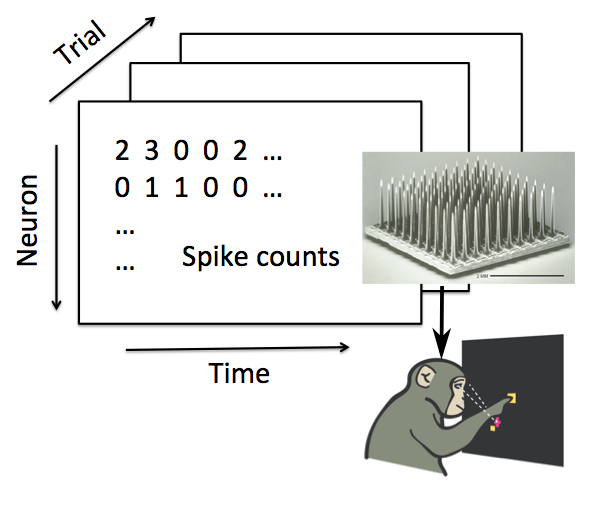
\includegraphics[width = 0.50\textwidth]{./figs/gclds/fig_monkey.png}
\begin{itemize}
\item Brain + Big data = \alert{Opportunities}!
\end{itemize}
\end{frame}


\begin{frame}
\frametitle{Table of Contents}
\tableofcontents
\end{frame}


\AtBeginSection[]
{
  \begin{frame}
    \frametitle{Table of Contents}
    \tableofcontents[
    currentsection, currentsubsection
]
  \end{frame}
}

\AtBeginSubsection[]
{
  \begin{frame}
    \frametitle{Table of Contents}
    \tableofcontents[
    currentsection, currentsubsection
]
  \end{frame}
}

%%%%%%%%%%%%%%%%%%%%%%% latent variable model for neural population data %%%%%%%%
\section[]{Neural Population Data Analysis with Latent Variable Models}

\begin{frame}
\frametitle{State space models}
\begin{figure}
\centering
{\small
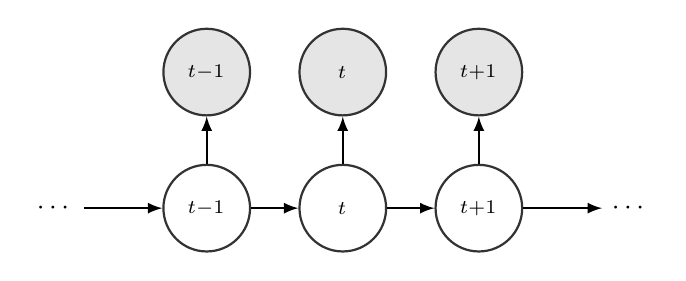
\begin{tikzpicture}
\tikzstyle{main}=[circle, minimum size = 11mm, thick, draw =black!80, node distance = 6mm]
\tikzstyle{connect}=[-latex, thick]
\tikzstyle{box}=[rectangle, draw=black!100]
  \node[main, fill = white!100] (z1) [] { $\vz_{t-1}$};
  \node[main] (z2) [right=of z1] {$\vz_{t}$ };
  \node[main] (z3) [right=of z2] {$\vz_{t+1}$};
  \node[main, fill = black!10] (x1) [above=of z1] { $\vx_{t-1}$};
  \node[main, fill = black!10] (x2) [above=of z2] {$\vx_{t}$ };
  \node[main, fill = black!10] (x3) [above=of z3] {$\vx_{t+1}$};
  \node (z0) [left=of z1] {$\cdots$};
  \node (zT) [right=of z3] {$\cdots$};
  \path (z1) edge [connect] (z2)
        (z2) edge [connect] (z3)
        (z1) edge [connect] (x1)
        (z2) edge [connect] (x2)
        (z3) edge [connect] (x3)
        (z0) edge [connect] (z1)
        (z3) edge [connect] (zT);
\end{tikzpicture}
}
\end{figure}
\begin{itemize}
\item $\vx_t \in \mathbb{N}^n$: spike counts; $\vz_t \in \mathbb{R}^m$: latent variables
%\item $p(\vx, \vz) = p(\vz_1) \prod_{t=1}^{T-1}p(\vz_{t+1} | \vz_t) \prod_{t=1}^T p(\vx_t | \vz_t)$
%\item Joint distribution
%\[\log p(\vx, \vz) = \underbrace{\log p(\vz_1)}_{\text{Initial distribution}} + 
%\underbrace{\sum_{t=1}^{T-1}\log p(\vz_{t+1} | \vz_t)}_{\text{Transition model}} + 
%\underbrace{\sum_{t=1}^T \log p(\vx_t | \vz_t)}_{\text{Observation model}}\]
\item Joint distribution
\[p(\vx, \vz) = \underbrace{p(\vz_1)}_{\text{Initial distribution}} 
\underbrace{\prod_{t=1}^{T-1}p(\vz_{t+1} | \vz_t)}_{\text{Transition model}} 
\underbrace{\prod_{t=1}^T p(\vx_t | \vz_t)}_{\text{Observation model}}\]
\item Common input; Dynamical view of motor data (TODO: elaborate this line)
\end{itemize}
\end{frame}


\begin{frame}
\frametitle{State space models: multiple trials}
\begin{figure}
\centering
{\footnotesize
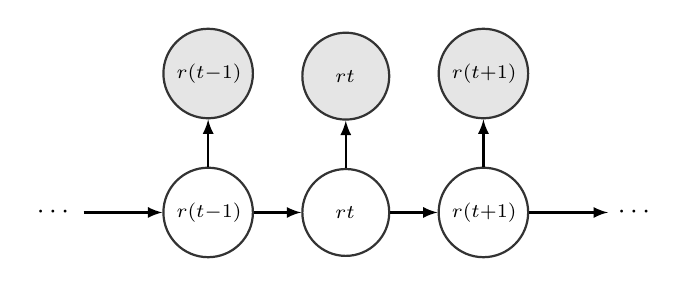
\begin{tikzpicture}
\tikzstyle{main}=[circle, minimum size = 11mm, text width = 8mm, align=center, thick, draw =black!80, node distance = 6mm]
\tikzstyle{connect}=[-latex, thick]
\tikzstyle{box}=[rectangle, draw=black!100]
  \node[main, fill = white!100] (z1) [] { $\vz_{r(t-1)}$};
  \node[main] (z2) [right=of z1] {$\vz_{rt}$ };
  \node[main] (z3) [right=of z2] {$\vz_{r(t+1)}$};
  \node[main, fill = black!10] (x1) [above=of z1] { $\vx_{r(t-1)}$};
  \node[main, fill = black!10] (x2) [above=of z2] {$\vx_{rt}$ };
  \node[main, fill = black!10] (x3) [above=of z3] {$\vx_{r(t+1)}$};
  \node (z0) [left=of z1] {$\cdots$};
  \node (zT) [right=of z3] {$\cdots$};
  \path (z1) edge [connect] (z2)
        (z2) edge [connect] (z3)
        (z1) edge [connect] (x1)
        (z2) edge [connect] (x2)
        (z3) edge [connect] (x3)
        (z0) edge [connect] (z1)
        (z3) edge [connect] (zT);
\end{tikzpicture}
}
\end{figure}
\begin{itemize}
\item $r=1,...,R$: trial number
\item $\vx_{rt} \in \mathbb{N}^n$: spike counts; $\vz_{rt} \in \mathbb{R}^m$: latent variables
%\item $p(\vx, \vz) = p(\vz_1) \prod_{t=1}^{T-1}p(\vz_{t+1} | \vz_t) \prod_{t=1}^T p(\vx_t | \vz_t)$
%\item Joint distribution
%\[\log p(\vx, \vz) = \underbrace{\log p(\vz_1)}_{\text{Initial distribution}} + 
%\underbrace{\sum_{t=1}^{T-1}\log p(\vz_{t+1} | \vz_t)}_{\text{Transition model}} + 
%\underbrace{\sum_{t=1}^T \log p(\vx_t | \vz_t)}_{\text{Observation model}}\]
\item Joint distribution
\[p(\vx, \vz) = \prod_{r=1}^R \left[ \underbrace{p(\vz_{r1})}_{\text{Initial distribution}} 
\underbrace{\prod_{t=1}^{T-1}p(\vz_{r(t+1)} | \vz_{rt})}_{\text{Transition model}} 
\underbrace{\prod_{t=1}^T p(\vx_{rt} | \vz_{rt})}_{\text{Observation model}} \right]\]
%\item Common input; Dynamical view of motor data (TODO: elaborate this line)
\end{itemize}
\end{frame}



\begin{frame}
\frametitle{Common parameterization and our extensions}
\begin{itemize}
\item Common assumptions for latent dynamics: linear Gaussian dynamical system (LDS)
 \[\begin{split}
 \vz_{1} &\sim \N(\mu_1, Q_1)\\
 \vz_{t+1} | \vz_{t} &\sim \N(A \vz_{t}, Q)
  \end{split}\]
\item Common observation models:
 \[\vx_t | \vz_t \sim \underbrace{\underbrace{\N(C \vz_t + d, \Sigma)}_{\text{model mismatch}}
 \text{ or }
 \underbrace{\text{Poisson}\left(\exp(C \vz_t + d)\right)}_{\text{equal dispersion}}}_\text{stringent assumptions}\]
\item Our extensions for observation model:
\begin{itemize}
\item Generalized count distribution (GCLDS) \parencite{Gao2015}
\item Flexible nonlinear observation (fLDS) \parencite{gao2016linear}
\end{itemize}
\end{itemize}
\end{frame}


%%%%%%%%%%%%%%%%%%%%%%% GCLDS %%%%%%%%
\subsection[]{Generalized count linear dynamical system}
\begin{frame}
\frametitle{Motivation}
\begin{itemize}
\item Doubly stochastic Poisson model implies \alert{overdispersion}
%\[ \vx \sim \text{Poisson}(f(\vz))  , \vz \sim p(\vz) \rightarrow \text{var}(\vx) \geq E(\vx)\]
\[\left. \begin{array}{ll} \vz &\sim p(\vz) \\ \vx &\sim \text{Poisson}(f(\vz)) \end{array} \right\} \Rightarrow \alert{\text{var}(\vx) \geq E(\vx)}\]
\item Need a more flexible distribution to separate \alert{firing rate variability} with \alert{noise variability}.
\[\text{var}(\vx) = \underbrace{\text{var}\left(E(\vx | \vz)\right)}_\text{firing rate variability} + \underbrace{E\left(\text{var}(\vx | \vz)\right)}_\text{noise variability}\]
\end{itemize}
\end{frame}


\begin{frame}
\frametitle{Generalized count distribution family}
\begin{itemize}
\item Generalized count (GC) distribution family
\[\begin{split}
p_{\text{Poisson}}(x; \lambda) \propto& \frac{\exp\left\{\log{\lambda} \cdot x\right\}}{x!},~~~x \in \mathbb{N}\\
\Downarrow&\\
p_{\mathcal{GC}}(x; \theta, g(\cdot)) \propto& \frac{\exp(\theta \cdot x + g(x) )}{x!}, ~~~x \in \mathbb{N}
\end{split}\]
where $\theta \in \mathbb{R}$, $g(\cdot): \mathbb{N} \rightarrow \mathbb{R}$.
\item Parameterizes \alert{all} the count distributions \alert{redundantly}.
\item Given $g(\cdot)$, $\theta$ controls the expectation.
\item $g(\cdot)$ controls the ``shape'' of the distribution. Convex/concave/linear $g(\cdot)$ implies overdispersed/underdispered/Poisson distribution.
\end{itemize}
\end{frame}


\begin{frame}
\frametitle{Model formulation}
 \begin{itemize}
 \item Linear dynamical systems with generalized count observation 
 \[\begin{split}
 \vz_{r1} &\sim \N(\mu_1, Q_1)\\
 \vz_{r(t+1)} | \vz_{rt} &\sim \N(A \vz_{rt}, Q)\\
 x_{rti} & \sim \mathcal{GC}(c_i^T \vz_{rt}, g_i(\cdot)), i = 1,...,n
 \end{split}\]
 \item Practical considerations
 \begin{itemize}
 %\item Set $g_i(0) = 0$ without loss of generality;
 \item Set $g_i(k) = -\infty$ for $k > K$ to facilitate computation;
 \item Ridge penalty on the $2^{\text{nd}}$ difference of $g_i(\cdot)$ to avoid overfitting;
 \item Set $g_i(0) = 0$ without loss of generality.
 \end{itemize}
 \end{itemize}
\end{frame}


\begin{frame}
\frametitle{Variational Bayes Expectation Maximization (VBEM)}
\begin{itemize}
\item $\vx$: data, $\vz$: latent variables, $\theta$: model parameters, 
\item Often hard to compute $p_\theta(\vx) = \int p_\theta(\vx, \vz) d \vz$ and $p_\theta(\vz | \vx)$.
\item Approximate the posterior by a \alert{tractable} distribution family.
\[p_{\theta}(\vz | \vx) \approx q(\vz) \in \mathcal{Q}\]
\item Optimize a \alert{lower bound of log likelihood}, or ELBO %w.r.t. both the model parameters and the variational distribution.
\[\begin{split}
&\text{ELBO}(\theta, q) = \int \left[\log p_{\theta}(\vx, \vz) - \log q(\vz)\right] q(\vz) d\vz \\
&= \log p_{\theta}(\vx) - \text{KL}(q(\vz) || p_\theta(\vz | \vx)) \leq \log p_{\theta}(\vx) % \log p_\theta(\vx) =& \log \int p_{\theta}(\vx, \vz) d \vz\\ 
\end{split}\]
%\[\begin{split}
%\log p_\theta(\vx) =& \log \int p_{\theta}(\vx, \vz) d \vz\\
%\geq& \int \left[\log p_{\theta}(\vx, \vz) - \log q(\vz)\right] q(\vz) d\vz
%\end{split}\]
\end{itemize}
\end{frame}

\begin{frame}
\frametitle{Variational Bayes Expectation Maximization (VBEM)}
\begin{itemize}
\item VBEM: Optimize $\text{ELBO}(\theta, q) \leq \log p_\theta(\vx)$ iteratively %by \alert{coordinate ascent}
\begin{itemize}
\item E-step: For a fixed $\theta$, optimize $q$ %(such that $q(\vz) \approx p_{\theta}(\vz | \vx)$)
\item M-step: For a fixed $q$, optimize $\theta$
%\item Iterate between E-step and M-step until convergence %, each iteration gives a higher ELBO and hopefully a higher log likelihood
\end{itemize}
\item VBEM for GCLDS 
\begin{itemize}
\item We set $q$ to be multivariate Gaussian
\item We derive a looser but tractable ELBO%The vanilla ELBO is still intractable, we use Jensen's inequality to get a tractable but looser bound. %(looser bound $\Rightarrow$ worse performance?)
%\item Fast initialization by Laplace approximation in .
\item E-step: fast Laplace approximation initialization + dual optimization
\item M-step: convex optimization + analytical solution
\end{itemize}
\end{itemize}
\end{frame}


\begin{frame}
\frametitle{Experiments}
\begin{itemize}
\item For both simulated and real dataset, we compare GCLDS with PLDS (Poisson observation model)
%\XSolid \Checkmark 
%\item On both simulated and real data
%GCLDS captures both mean and variance of the data well, PLDS capture 
\begin{center}
\begin{tabular}{ cccc } 
 \hline
  & Mean & Variance & \alert{Likelihood} \\
 \hline
 PLDS & \cmark & \xmark& \xmark \\ 
 \alert{GCLDS} &\cmark &\cmark &\cmark \\ 
 \hline
\end{tabular}
\end{center}
\end{itemize}
\end{frame}


\begin{frame}
\frametitle{Real data analysis: data}
\begin{tabular}{ cc } 
{\small Data} & {\small Variance and mean of spike counts}\\
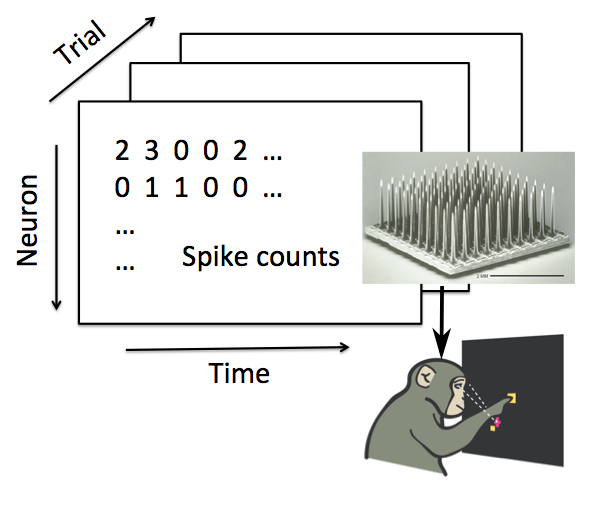
\includegraphics[width = 0.40\textwidth]{./figs/gclds/fig_monkey.png}&
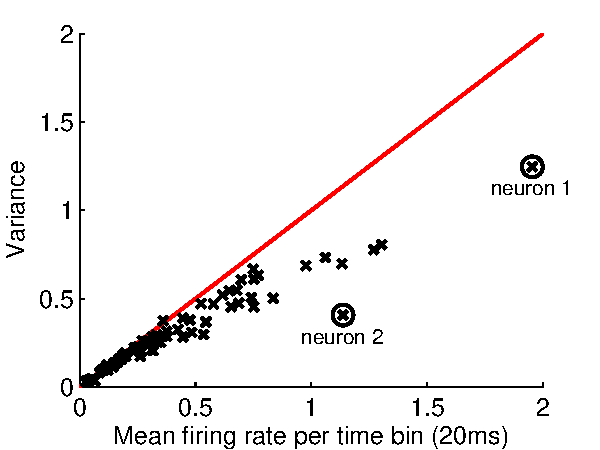
\includegraphics[width = 0.45\textwidth]{./figs/gclds/fig_var_obs_Move_seq14.pdf}
\end{tabular}
\begin{itemize}
\item Center-out reaching experiments
\item Multi-electrode array recording
\item Strong \alert{under-dispersion}
\end{itemize}
\end{frame}


\begin{frame}
\frametitle{Real data analysis: algorithms}
\begin{itemize}
\item Main algorithms to be compared
\begin{itemize}
\item \alert{PLDS}: Poisson observation
\item \alert{GCLDS-full}: Generalized count observation, individual $g(\cdot)$ across neurons
\end{itemize}
\item Two control cases for GCLDS
\begin{itemize}
\item \alert{GCLDS-linear}: truncated linear $g(\cdot)$ (truncated Poisson)
\item \alert{GCLDS-simple}: $g(\cdot)$ shared across neurons (up to a linear function)
\end{itemize}
\end{itemize}
\end{frame}


\begin{frame}
\frametitle{Real data analysis: single neuron fit}
\begin{tabular}[t]{ccc}
{\small Fitted $g(\cdot)$} & {\small Fitted mean} & {\small Fitted variance}\\
		\raisebox{-0.85\totalheight}{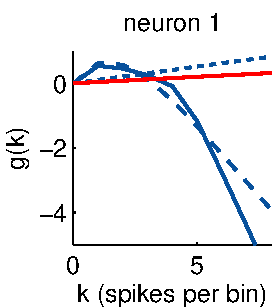
\includegraphics[scale=0.5,clip = true]{figs/gclds/fig_962346_seq14_xDim8_neu1_g.pdf}}&
		\raisebox{-0.85\totalheight}{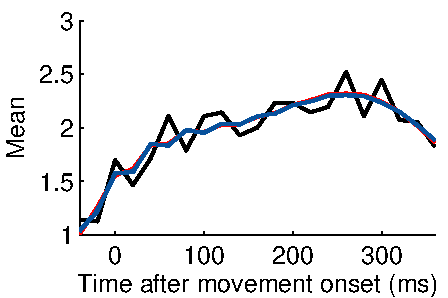
\includegraphics[scale=0.5,clip = true]{figs/gclds/fig_962346_seq14_xDim8_neu1_mean.pdf}}&
		\raisebox{-0.85\totalheight}{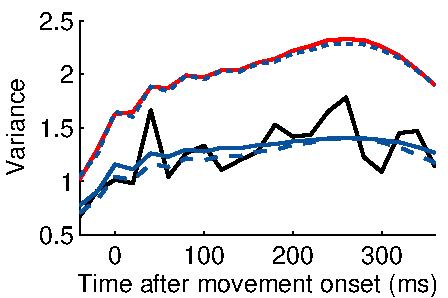
\includegraphics[scale=0.5,clip = true]{figs/gclds/fig_962346_seq14_xDim8_neu1_var.pdf}}\\

		%B)&\raisebox{-0.85\totalheight}{\includegraphics[width=0.3\textwidth,clip = true]{figs/fig_gclds/fig_1625526_seq14_xDim8_neu2_g.pdf}}&
		%\raisebox{-0.85\totalheight}{\includegraphics[width=0.3\textwidth,clip = true]{figs/fig_gclds/fig_1625526_seq14_xDim8_neu2_mean.pdf}}&
		%\raisebox{-0.85\totalheight}{\includegraphics[width=0.3\textwidth,clip = true]{figs/fig_gclds/fig_1625526_seq14_xDim8_neu2_var.pdf}}\\
		\raisebox{-0.85\totalheight}{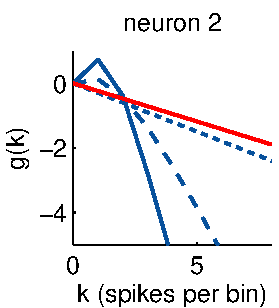
\includegraphics[scale=0.5,clip = true]{figs/gclds/fig_962346_seq14_xDim8_neu3_g.pdf}}&
		\raisebox{-0.85\totalheight}{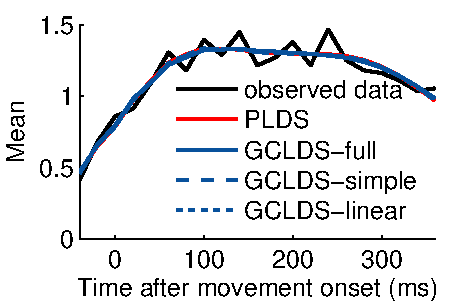
\includegraphics[scale=0.5,clip = true]{figs/gclds/fig_962346_seq14_xDim8_neu3_mean.pdf}}&
		\raisebox{-0.85\totalheight}{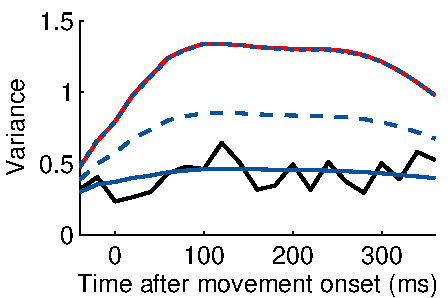
\includegraphics[scale=0.5,clip = true]{figs/gclds/fig_962346_seq14_xDim8_neu3_var.pdf}}\\
				%&{\graphFont Dates}&\\
\end{tabular}
\end{frame}

\begin{frame}
\frametitle{Real data analysis: population fit}
%\begin{centering}
\begin{itemize}
\item Leave-one-neuron-out prediction
%\begin{itemize}
%\item Separate trials into training and testing
%\item Use training data to learn parameters
%\item For test data, drop one neuron and use other neurons to predict its firing rate
%\end{itemize}
\end{itemize}
\begin{center}
\begin{tabular}[t]{cc}
{\small MSE reduction} & {\small NLL reduction} \\
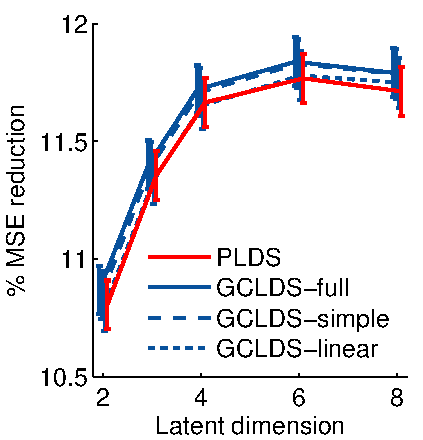
\includegraphics[scale=0.5,clip = true]{figs/gclds/fig_MSE_band_George_Move_NULL.pdf}&
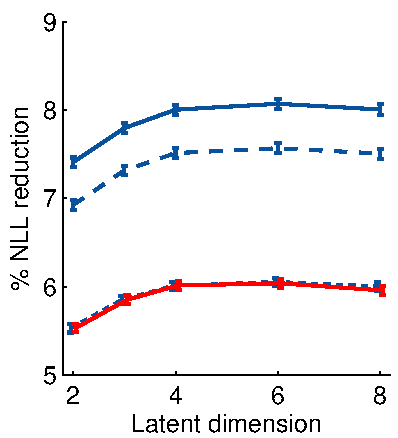
\includegraphics[scale=0.5,clip = true]{figs/gclds/fig_likelihood_band_George_Move_NULL.pdf}%&
%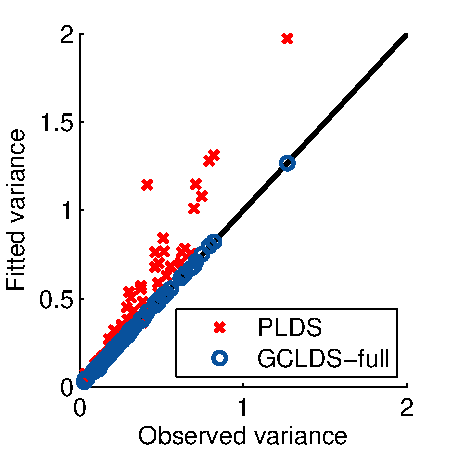
\includegraphics[scale=0.43,clip = true]{figs/gclds/fig_var_JOB962346_seq14_xDim8_plot.pdf}
\end{tabular}
\end{center}
%\end{centering}
\end{frame}



\begin{frame}
\frametitle{Conclusion and discussion}
\begin{itemize}
\item Summary
\begin{itemize}
\item Incorporated generalized count family into state space models.
\item Developed VBEM algorithm.
\item Observed superior fitted result on real neural data.
\end{itemize}
\item Extensions
\begin{itemize}
\item $g(\cdot)$ vary across time?
\item Share information of $g(\cdot)$ across neurons? (hierarchical model?)
\item Generative models for under-dispersion?
\end{itemize}
\item \alert{Gao Y}, Buesing L, Shenoy KV, Cunningham JP (2015) High-dimensional neural spike train analysis with generalized count linear dynamical systems. NIPS 2015.
\end{itemize}
\end{frame}



%%%%%%%%%%%%%%%%%%%%%%% fLDS %%%%%%%%
\subsection[]{Linear dynamical neural population models through nonlinear embeddings}

\begin{frame}
\frametitle{Motivation}
\begin{tabular}{cl}
\parbox{0.6\textwidth}{
\begin{itemize}
\item Neural activities lie in a low-dimensional \alert{nonlinear manifold} rather than a \alert{linear subspace}
\item Flexible observation model makes the state space model more expressive
\end{itemize}
}
&
\hspace{-1cm}
\begin{tabular}{c}
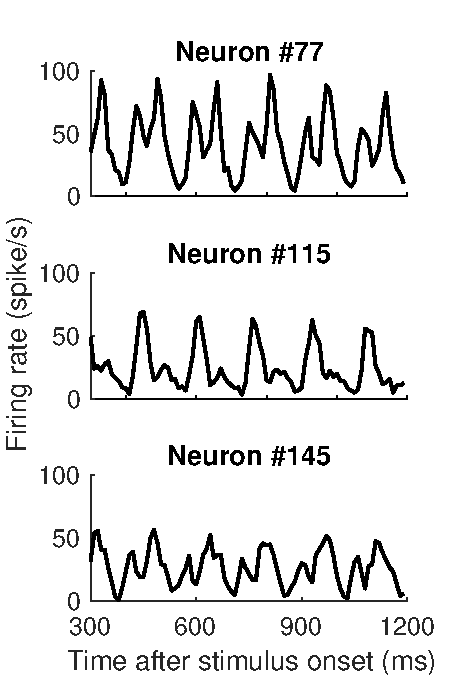
\includegraphics[scale=0.5,clip = true]{figs/flds/fig_V1_single_3concat_onlyobservation.pdf}
\end{tabular}
\end{tabular}
\end{frame}


\begin{frame}
\frametitle{Model formulation: fLDS}
\begin{itemize}
 \item Linear dynamical systems with \alert{nonlinear link} and count observation
 \[\begin{split}
 \vz_{r1} \sim& \N(\mu_1, Q_1)\\
 \vz_{r(t+1)} | \vz_{rt} \sim& \N(A \vz_{rt}, Q)\\
 x_{rti} \sim& \text{Poisson}(\alert{f}_i(\vz_{rt})) \text{ (PfLDS) } \\
 &\text{   or }\mathcal{GC}(\alert{f}_i(\vz_{rt}), g_i(\cdot)) \text{ (GCfLDS)}%, i = 1,...,n
 \end{split}\]
 where $f_i$ is a nonlinear function parameterized by a neural network
 \item Linear dynamics: simple, tractable, interpretable
 \item Nonlinear observation: flexibility
\end{itemize}
\end{frame}

\begin{frame}
\frametitle{Inference algorithm: AEVB (high level idea)}
%\begin{itemize}
%\item Auto-encoding Variational Bayes (AEVB)
\begin{itemize}
\item Auto-encoding Variational Bayes (AEVB)
\item Learn a mapping (recognition model) from data to the \alert{approximate posterior distribution of latent variable}.
\item Jointly optimize the generative model parameters and recognition model parameters.
\item Naturally incorporate stochastic optimization to handle large datasets.
\end{itemize}
%\end{itemize}
\end{frame}

\begin{frame}
\frametitle{Inference algorithm: AEVB (algorithm)}
\begin{itemize}
\item Decompose ELBO by trials
\[\begin{split}
\text{ELBO}(\theta, q) %=& \int \left[\log p_{\theta}(\vx, \vz) - \log q(\vz)\right] q(\vz) d\vz\\
=& \sum_{r=1}^{R} \int \left[\log p_{\theta}(\vx_r, \vz_r) - \log q(\vz_r)\right] q(\vz_r) d\vz_r 
\end{split}\]
\item Map data $\vx_r$ to $q(\vz_r)$ by a parameterized function
\[q(\vz_r) = q_\phi(\vz_r; \vx_r) = \N\left(\mu_\phi(\vx_r), \Sigma_\phi(\vx_r)\right)\]
\item Learn both $\theta$ and $\phi$ by optimizing ELBO
\[\text{ELBO}(\theta, \phi) = \sum_{r=1}^{R} \int \left[\log p_{\theta}(\vx_r, \vz_r) - \log q_\phi(\vz_r; \vx_r)\right] q_\phi(\vz_r; \vx_r) d\vz_r \]
\item Do stochastic optimization with gradient of a single trial
\end{itemize}
\end{frame}


\begin{frame}
\frametitle{Inference algorithm: AEVB (important details)}
\begin{itemize}
\item Specific parameterization of the recognition model
\[q(\vz_r) = q_\phi(\vz_r; \vx_r) = \N\left(\mu_\phi(\vx_r), \Sigma_\phi(\vx_r)\right)\]
\vspace{-0.5cm}
\begin{itemize}
\item Block tri-diagonal precision matrix that agrees with Markovian structure
\item Potentially useful to perform filtering in an online fashion
\end{itemize}
\item Reparameterization trick for stochastic optimization
\begin{itemize}
\item Easy implementation
\item Low variance
\end{itemize}
\end{itemize}
\end{frame}

\begin{frame}
\frametitle{Experiments}
\begin{center}
\begin{tabular}{ ccccc } 
 \hline
  & Mean & Variance & Likelihood & \alert{Concise representation}\\
 \hline
 PLDS & \cmark & \xmark& \xmark &  \xmark  \\ 
 GCLDS &\cmark &\cmark &\cmark &  \xmark  \\ 
 \alert{PfLDS} & \cmark & \xmark& \xmark &   \cmark\\ 
 \alert{GCfLDS} &\cmark &\cmark &\cmark &  \cmark \\ 
 \hline
\end{tabular}
\end{center}
\end{frame}

\begin{frame}
\frametitle{Real data analysis: primate visual cortex}
%\hspace{-1cm}
\begin{tabular}{cc}
\small{Firing rate} & \\
\begin{tabular}{c}
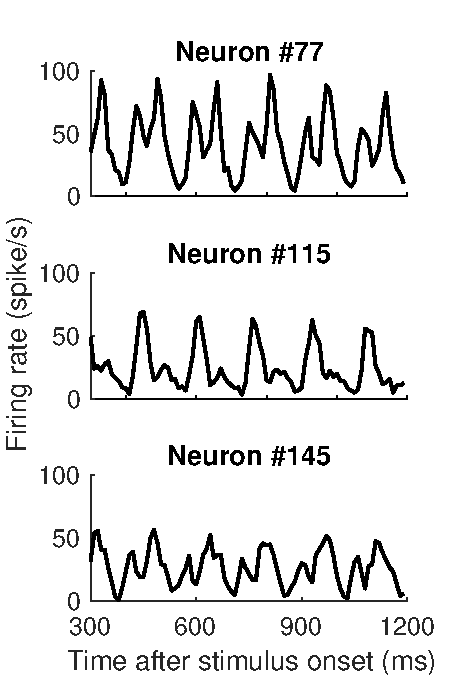
\includegraphics[scale=0.45,clip = true]{figs/flds/fig_V1_single_3concat_onlyobservation.pdf} 
\end{tabular}
&
\begin{tabular}{c}
%PLDS \\
%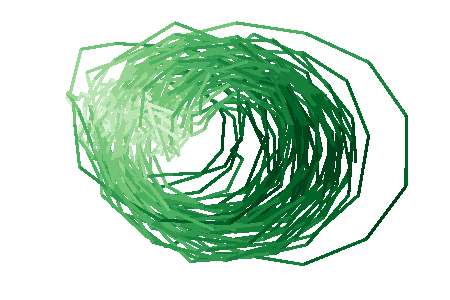
\includegraphics[scale=0.5,clip = true]{figs/flds/fig_V1_mat_trajectory_3concat.pdf}\\
%PfLDS \\
%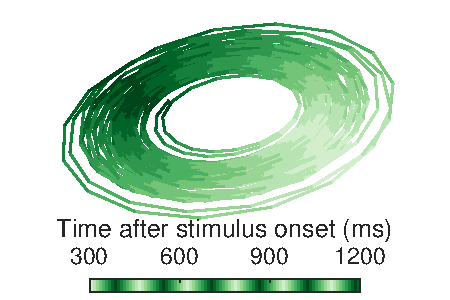
\includegraphics[scale=0.5,clip = true]{figs/flds/fig_V1_py_trajectory_3concat.pdf}
\end{tabular}
\end{tabular}
\end{frame}



\begin{frame}
\frametitle{Real data analysis: primate visual cortex}
%\hspace{-1.2cm}
\begin{tabular}{ccc}
{\small \visible<1->Firing rate} & \visible<2->{\hspace{-0.6cm}\small{Latent projection}} & \visible<3->{\hspace{-0.6cm}\small{1-step-ahead prediction}}\\
%\hline
\begin{tabular}{c}
\visible<1->{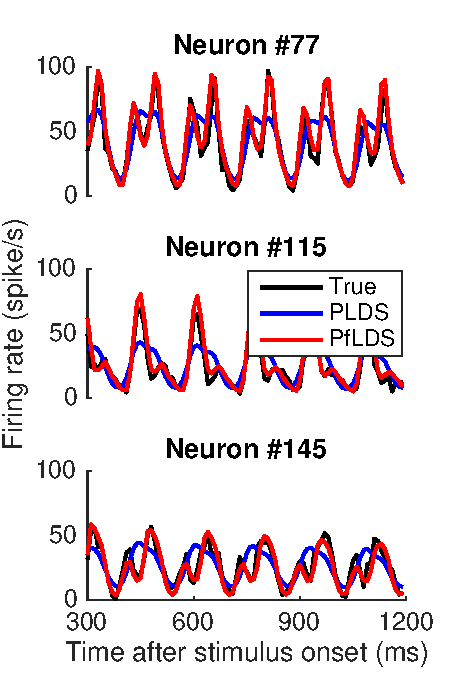
\includegraphics[scale=0.45,clip = true]{figs/flds/fig_V1_single_3concat.pdf}}
%\visible<2->{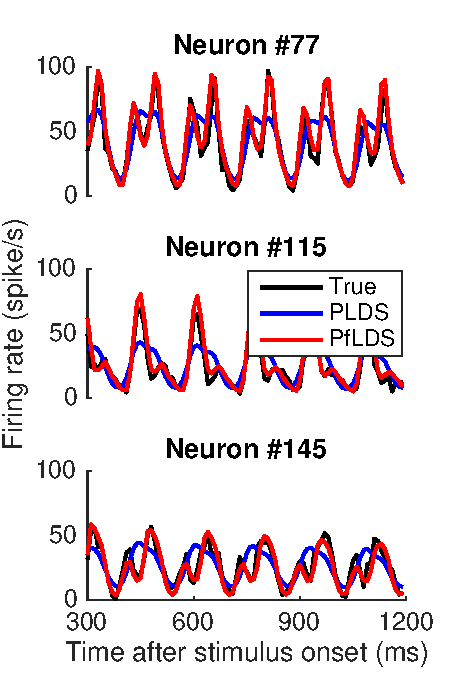
\includegraphics[scale=0.5,clip = true]{figs/flds/fig_V1_single_3concat.pdf} }
\end{tabular}
&
\hspace{-0.6cm}
\begin{tabular}{c}
\visible<2->{\scriptsize{PLDS} \\
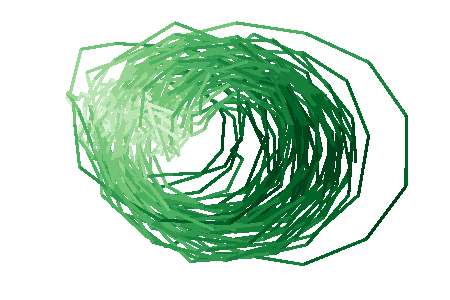
\includegraphics[scale=0.4,clip = true]{figs/flds/fig_V1_mat_trajectory_3concat.pdf}\\
\scriptsize{PfLDS} \\
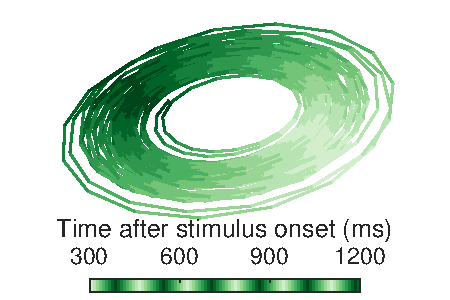
\includegraphics[scale=0.4,clip = true]{figs/flds/fig_V1_py_trajectory_3concat.pdf}}
\end{tabular}
&
\hspace{-0.6cm}
\visible<3->{\begin{tabular}{c}
\scriptsize{MSE reduction}\\
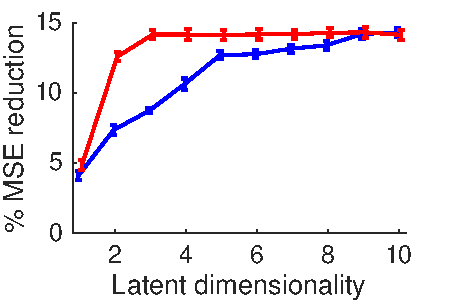
\includegraphics[scale=0.40,clip = true, trim = 0cm 0cm 0cm 0.2cm]{figs/flds/fig_V1_MSE_3concat.pdf}\\
\scriptsize{NLL reduction}\\
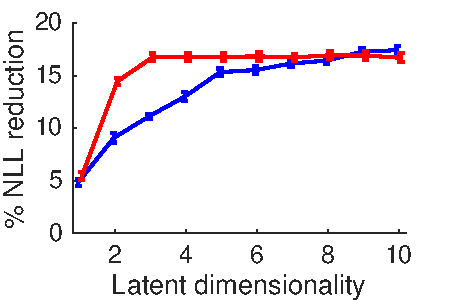
\includegraphics[scale=0.40,clip = true, trim = 0cm 0cm 0cm 0.2cm]{figs/flds/fig_V1_NLL_3concat.pdf}\\
\end{tabular}}
\end{tabular}
\end{frame}


\begin{frame}
\frametitle{Real data analysis: Primate motor cortex}
\begin{tabular}{ cc } 
{\small Data} & {\small Reaching trajectory} \\
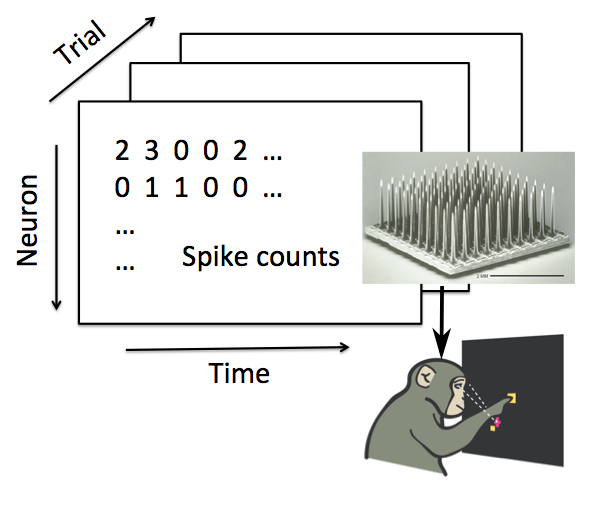
\includegraphics[width = 0.45\textwidth]{./figs/gclds/fig_monkey.png}&
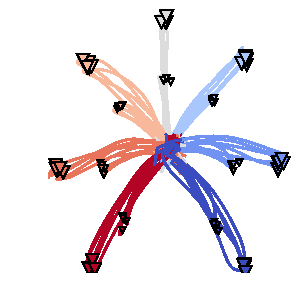
\includegraphics[width = 0.40\textwidth]{./figs/flds/fig_GeorgeMove_trajectory.pdf}
\end{tabular}
\end{frame}


\begin{frame}
\frametitle{Real data analysis: Primate motor cortex}
\begin{itemize}
\item Latent projection with $2$ latent dimensions
\end{itemize}
\begin{tabular}{ ccc } 
{\small Reaching trajectory} & {\small PLDS} & {\small PfLDS} \\
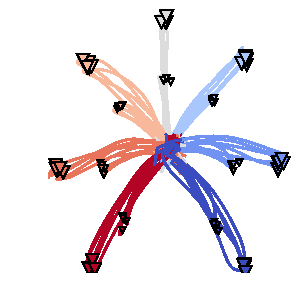
\includegraphics[width = 0.30\textwidth]{./figs/flds/fig_GeorgeMove_trajectory.pdf}&
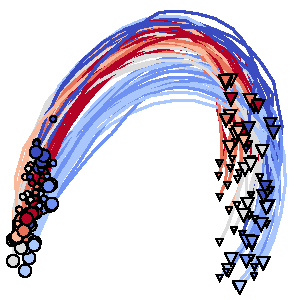
\includegraphics[width = 0.30\textwidth]{./figs/flds/fig_GeorgeMove_2dvisual_mat_PLDS.pdf}&
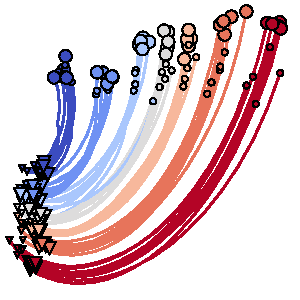
\includegraphics[width = 0.30\textwidth]{./figs/flds/fig_GeorgeMove_2dvisual_py_PLDS.pdf}
\end{tabular}
\end{frame}

\begin{frame}
\frametitle{Real data analysis: Primate motor cortex}
\begin{itemize}
\item One-step-ahead predictive performance
\end{itemize}
\begin{center}
\begin{tabular}{ cc} 
{\small MSE reduction} & {\small NLL reduction}\\
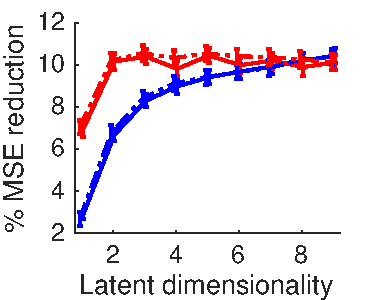
\includegraphics[scale = 0.6]{./figs/flds/fig_GeorgeMove_MSE_GC.pdf}&
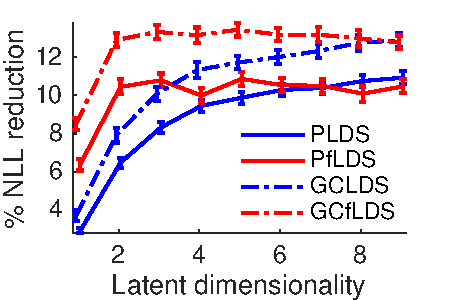
\includegraphics[scale = 0.6]{./figs/flds/fig_GeorgeMove_NLL_GC.pdf}
\end{tabular}
\end{center}
\end{frame}


\begin{frame}
\frametitle{Conclusion and discussion}
\begin{itemize}
\item Summary
\begin{itemize}
\item Incorporated nonlinear observation into state space models.
\item Developed AEVB algorithm (flexible and scalable).
\item Obtain concise latent representation.
\end{itemize}
\item Future work
\begin{itemize}
\item Better stochastic optimization scheme
\item Interpretable nonlinearity
\item Application on more complex datasets
\end{itemize}
\item \alert{Gao Y}*, Archer E*, Paninski L, Cunningham JP (2016) Linear dynamical neural population models through nonlinear embeddings. NIPS 2016. (* = equal contribution)
\end{itemize}
\end{frame}


%%%%%%%%%%%%%%%%%%%%%% ROI detection %%%%%%%%%%%%%%%%%%%%%%%%%
\section[]{Region of Interest Detection for Calcium Imaging Data}

\begin{frame}
\frametitle{Introduction: calcium imaging data}
TODO: incorporate a video?
\end{frame}

\begin{frame}
\frametitle{Model formulation: idea}
\begin{itemize}
\item  $X \in \mathbb{R}^{N \times T}$ represents the calcium imaging data, where each column is a (vectorized) frame that contains $N$ pixels
\item Decompose $X$ into a product of $K$ \alert{spatial component} and \alert{temporal component}% (neural acitivities)
\[X = D \cdot A^T + \text{noise}\]
\begin{itemize}
\item $D = [D_1,...,D_K] \in \mathbb{R}^{N \times K}$ represents the neuron shapes
\item $A = [A_1,...,A_K] \in \mathbb{R}^{T \times K}$ is the neural activities%, $K$ is the number of neurons.
\end{itemize}
\item Further exploit structure of the components (localized neuron shapes)
\end{itemize}
\end{frame}

\begin{frame}
\frametitle{Model formulation: objective}
\begin{itemize}
\item Structured matrix factorization
\[
%\label{equ:opt}
\begin{aligned}
& \underset{D, A}{\text{minimize}}
& & \| X - D A^T \|_2^2 + f_D(D), \\
& \text{subject to}
& & D_k \in \mathcal{D}_{w}^+; k = 1, \ldots, K,\\
& 
& & \|A_k\|_2 \leq c_k,
\end{aligned}
\]
\item $\mathcal{D}_{w}^+$: non-negative vectors whose nonzero values is within a $w \times w$ window
\item $f_D(D)$ regularizes the neuron shape (discussed later)
\item $\|A_k\|_2 \leq c_k$ avoids degenerate solution
\end{itemize}
\end{frame}


\begin{frame}
\frametitle{Greedy algorithm}
\begin{itemize}
\item Scan the each frame of the video with a small Gaussian kernel
\item At iteration $k$, given the current residue (unexplained by existing ROI)
\begin{itemize}
\item \alert{Greedy identification}: Identify the location $p_k$ where the Gaussian kernel explains most of the data (across time)
\item \alert{Shape fine tuning}: Locally optimize the spatial and temporal component
\item \alert{Residue update}: Subtract the newly identified ROI
\end{itemize}
\end{itemize}
\end{frame}


\begin{frame}
\frametitle{Shape fine tuning}
\begin{itemize}
\item Given current residue $R$, an identified center pixel $p_k$, denote $S_k$ as a $w \times w$ window centered at $p_k$
\[
\begin{aligned}
& \underset{D_k, A_k}{\text{minimize}}
& & \| R - D_k A_k^T \|^2 + f(D_k), \\%\sum_{i = 1}^3 \lambda_i f_i(D_k),\\
& \text{subject to}
& & D_{kp} \geq 0, p \in S_k,\\
&
& & D_{kp} = 0, p \notin S_k,\\
& 
& & \|A_k\|_2 \leq c_k,
\end{aligned}
\]
%\begin{itemize}
\item $f(D_k) = \sum_{i=1}^3 \lambda_i f_i(D_k)$
%where
\begin{itemize}
\item $f_1(D_k) = \sum_p \tau_{(p, p_k)} | D_{kp} |$ encourages sparsity
\item $f_2(D_k) = \sum_p (D_{kp} - G_{p_k})^2$ encourage Gaussian shape
\item $f_3(D_k) = \sum_{\text{$p_1$ and $p_2$ are neighbors}} (D_{kp_1} - D_{kp_2})^2$ encourages smoothness
\end{itemize}
\item Optimize $D_k$ and $A_k$ by block coordinate descent
%\item Need to tune regularization parameters, not necessarily good since those would shrink the estimated shape
\end{itemize}
%\end{itemize}
\end{frame}

\begin{frame}
\frametitle{Real data analysis: sample patch, no shape regularization}
\begin{tabular}[t]{cc}
%\multicolumn{2}{c}{Gaussian kernel shape}  \\
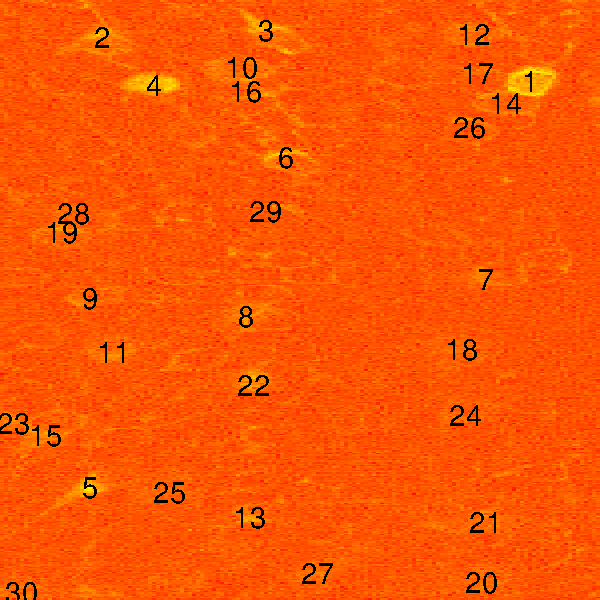
\includegraphics[scale=0.35,clip = true]{figs/ROI/fig_Misha_plain_comp.pdf}&
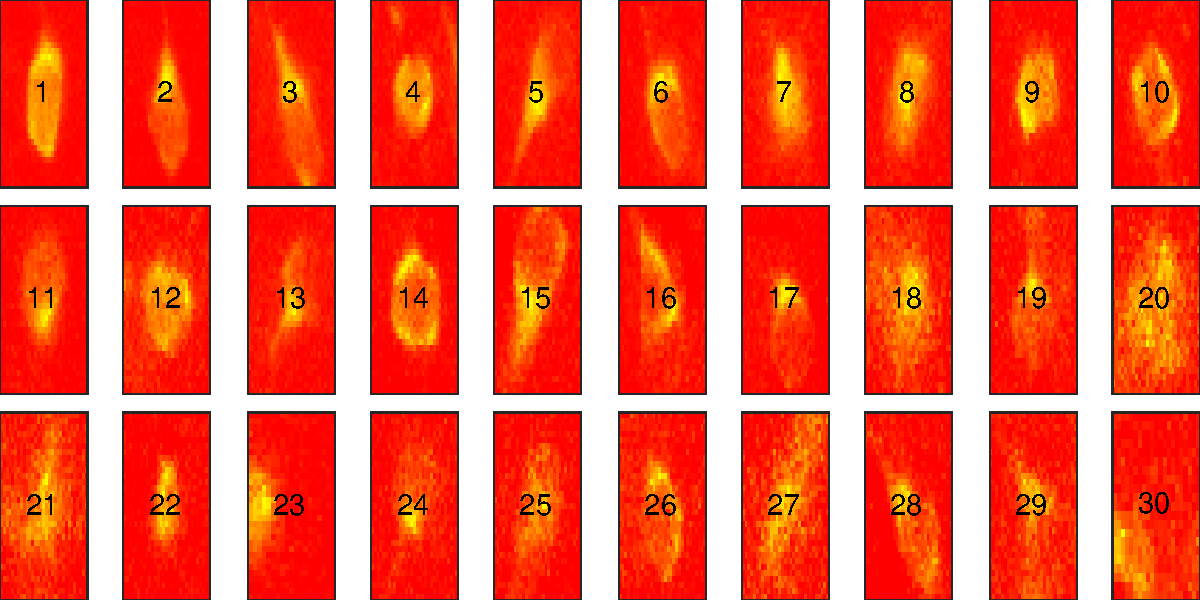
\includegraphics[scale=0.35,clip = true]{figs/ROI/fig_Misha_plain_shape.pdf}\\
%\multicolumn{2}{c}{Ring shape} \\
%\includegraphics[scale=0.45,clip = true]{figs/fig_ROI/fig_simulation_comp_Ring.pdf}&
%\includegraphics[scale=0.45,clip = true]{figs/fig_ROI/fig_simulation_shape_Ring.pdf}\\
%\\
\end{tabular}
\end{frame}

\begin{frame}
\frametitle{Real data analysis: sample patch, shape regularization}
\begin{tabular}[t]{cc}
%\multicolumn{2}{c}{Gaussian kernel shape}  \\
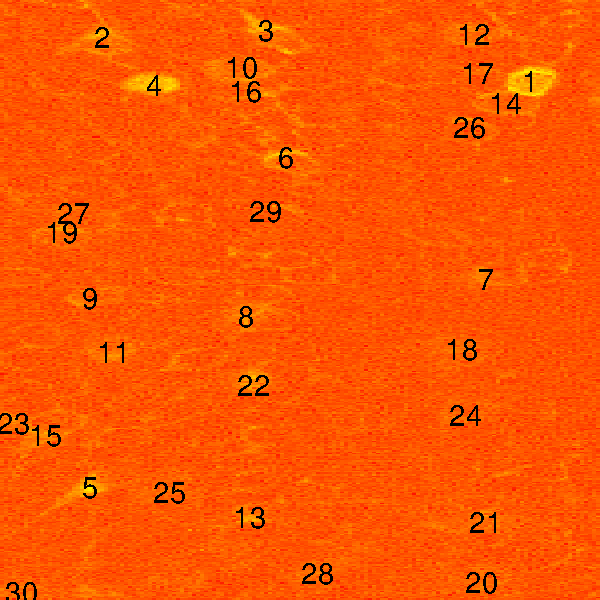
\includegraphics[scale=0.35,clip = true]{figs/ROI/fig_Misha_smooth_comp.pdf}&
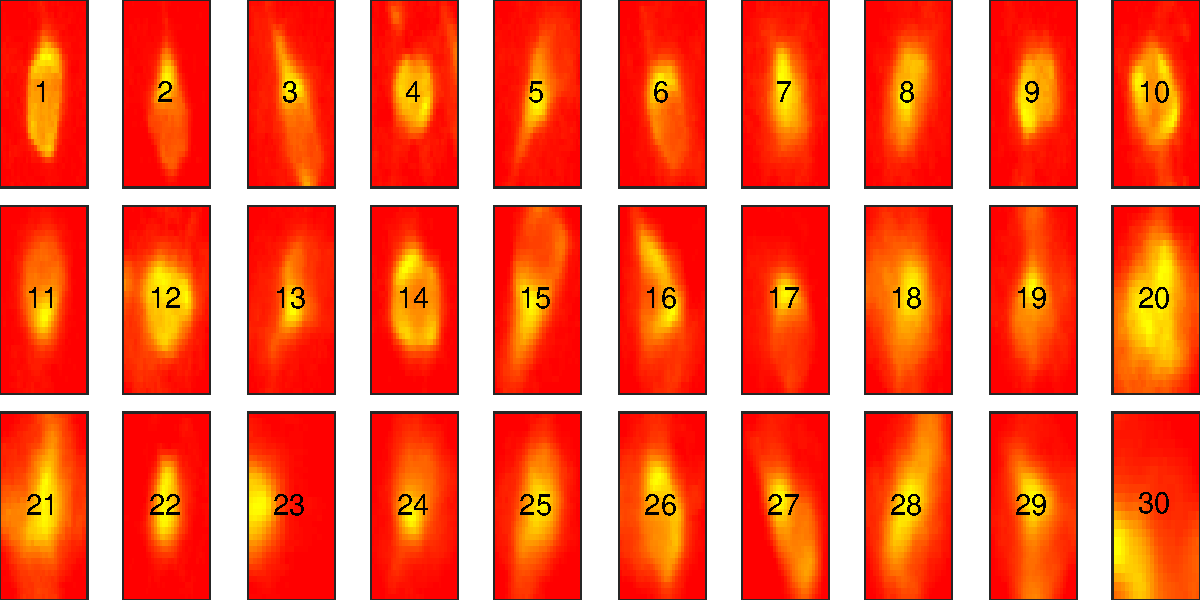
\includegraphics[scale=0.35,clip = true]{figs/ROI/fig_Misha_smooth_shape.pdf}\\
%\multicolumn{2}{c}{Ring shape} \\
%\includegraphics[scale=0.45,clip = true]{figs/fig_ROI/fig_simulation_comp_Ring.pdf}&
%\includegraphics[scale=0.45,clip = true]{figs/fig_ROI/fig_simulation_shape_Ring.pdf}\\
%\\
\end{tabular}
\end{frame}


\begin{frame}
\frametitle{Conclusion and discussion}
\begin{itemize}
\item Summary
\begin{itemize}
\item Formulating calcium imaging ROI detection as a structure matrix factorization problem
\item Greedy algorithm with shape regularization
\item Fast ROI detection algorithm
\end{itemize}
\item Future work
\begin{itemize}
\item More spatial and temporal structure
\item Overlapping neuron
\item Online ROI detection
\item Motion correction, background elimination
\end{itemize}
\item {\scriptsize Pnevmatikakis EA, Soudry D, \alert{Gao Y}, Machado TA, Merel J, Pfau D, Reardon T, Mu Y, Lacefield C, Yang W, Ahrens M, Bruno R, Jessell TM, Peterka DS, Yuste R, Paninski L (2016) Simultaneous denoising, deconvolution, and demixing of calcium imaging data. Neuron, 89(2), 285-299.}
\end{itemize}
\end{frame}


%%%%%%%%%%%%%%%%%%%%% MEFN %%%%%%%%%%%%%%%%%%%%%%%%%%%%%
\section[]{Maximum Entropy Flow Networks}

\begin{frame}
\frametitle{Maximum entropy principle}
\begin{itemize}
\item \alert{Entropy}: for a continuous distribution with density $p(\vz)$ where $\vz \in \mathbb{R}^d$, the entropy is defined as
\[H(p) = - \int p(\vz) \log p(\vz)  d \vz = E_{Z \sim p} \left[ -\log p(Z) \right].\]
A popular measure of diversity or information content.
\item \alert{Maximum entropy (ME) principle}: Subject to some given prior knowledge (moment or support constraints), the distribution that makes \alert{minimal additional assumptions} is that which has the \alert{largest entropy} of any distribution obeying those constraints
\end{itemize}
\end{frame}

\begin{frame}
\frametitle{Maximum entropy problem}
\begin{itemize}
\item Maximum entropy (ME) problem
\begin{eqnarray*}
%\substack{E_{\mZ\sim p}[T(\mZ)]=0 \\ \supp(p)=\mathcal{X}}
p^{*} &=& \text{maximize}~~~ H(p) \\
&& \text{subject to} ~~~E_{\mZ\sim p}[T(\mZ)]=0 \nonumber\\
&& ~~~~~~~~~~~~~~~~~~\supp(p)=\mathcal{Z} \nonumber,
\end{eqnarray*}
where $T(\vz) = (T_1(\vz),...,T_m(\vz)):\mathcal{Z}\rightarrow \mathbb{R}^{m}$ is the vector of known statistics, and $\mathcal{Z}$ is the given support.
%\item Useful for model formulation and hypothesis testing.
%\item \alert{Problem}: hard to learn and sample from maximum entropy distribution when constraints are complicated
\end{itemize}
\end{frame}

\begin{frame}
\frametitle{Applications of maximum entropy}
\begin{itemize}
\item \alert{Texture modeling}: generate an image with a certain texture by specifying expected value of features relevant to texture.
\item \alert{Neuroscience}: generate a distribution of neural activity by specifying a set of features (pairwise correlation etc.) for hypothesis testing.
\item \alert{Ecology}: Fit species distribution with certain feature constraints (altitude, temperature etc.).
\item \alert{Finance}: Fit the risk-neutral distribution of an asset given a list of option prices.
\item ...
\end{itemize}
\end{frame}

\begin{frame}
\frametitle{Gibbs distribution}
\begin{itemize}
\item Under standard regularity conditions, the maximum entropy problem can be solved by Lagrange multipliers, yielding an exponential family $p^*$ of the form (Gibbs distribution):
\[\label{curmet}
p^*(\vz) \propto e^{<\eta, T(\vz)>} \mathbbm{1}(\vz \in \mathcal{Z})
\]
\item Identifying $\eta \in \mathbb{R}^m$ can be hard in high-dimensional setting.
\item Sampling from the distribution can be hard. MCMC methods can take long to mix.
\item \alert{Question}: is there a better way to do this?
\end{itemize}
\end{frame}


\begin{frame}
\frametitle{Idea: normalizing flow}
\begin{itemize}
\item Considering a family of smooth and invertible transformation (\alert{normalizing flow}) \[\mathcal{F}=\{f_\phi:  \mathbb{R}^d \rightarrow \mathbb{R}^d, \phi \in \mathbb{R}^q\}\]
\item Identify a transformation $f_{\phi^*} \in \mathcal{F}$ that transforms a simple distribution $p_0$ to approximate the maximum entropy distribution.
\begin{eqnarray*}\label{optobj}
%\substack{E_{\mZ\sim p}[T(\mZ)]=0 \\ \supp(p)=\mathcal{X}}
\phi^{*} &=& \text{maximize}~~~ H(p_\phi) \\
&& \text{subject to} ~~~E_{\mZ_0\sim p_0}[T(f_\phi(\mZ_{0}))]=0 \nonumber\\
&& ~~~~~~~~~~~~~~~~~~\supp(p_\phi)=\mathcal{Z}. \nonumber
\end{eqnarray*}
where $p_\phi(\vz)$ is the distribution of $f_\phi(Z_0)$ for $Z_0 \sim p_0$.
\[p_\phi(\vz) = p_0( f_\phi^{-1}(\vz) ) | \det (J_\phi (\vz)) |^{-1}\]
\end{itemize}
\end{frame}


\begin{frame}
\frametitle{Augmented Lagrangian method}
\begin{itemize}
\item Denote $R(\phi) = E\left(T(f_\phi( \mZ_0))\right) \in \mathbb{R}^m$, augmented Lagrangian method minimizes the objective
\[L(\phi; \lambda, c) = - H(p_\phi) + \lambda^{\top} R(\phi) + \dfrac{c}{2}||R(\phi)||^2\]
for a sequence of $\lambda \in \mathbb{R}^m$ and $c \geq 0$.
\item Update rule: at iteration $k$, given $\lambda_k$ and $c_k$, suppose $\phi_k$ optimizes $L(\phi; \lambda_k, c_k)$, update $\lambda$ and $c$ by
\[\begin{split}
\lambda_{k+1} =& \lambda_k + c_k R(\phi_k)\\
c_{k+1} =&\begin{cases}
\beta c_{k} & ||R(\phi_{k})||>\gamma ||R(\phi_{k-1})|| \\
c_k & \text{otherwise}
\end{cases}
\end{split}\]
for some $\gamma \in (0,1)$, $\beta > 1$
\end{itemize}
\end{frame}

\begin{frame}
\frametitle{Augmented Lagrangian method in stochastic setting}
\begin{itemize}
\item Denote $R(\phi) = E\left(T(f_\phi( \mZ_0))\right) \in \mathbb{R}^m$, augmented Lagrangian method minimizes the objective
\[L(\phi; \lambda, c) = - H(p_\phi) + \lambda^{\top} R(\phi) + \dfrac{c}{2}||R(\phi)||^2\]
for a sequence of $\lambda \in \mathbb{R}^m$ and $c \geq 0$.
\item Here $R(\phi) = E\left(T(f_\phi( \mZ_0))\right) \in \mathbb{R}^m$ is intractable, but we can approximate with a sampled version.
\[R(\phi) \approx \frac{1}{n} \sum_{i=1}^nT(f_\phi( \vz^{(i)})), \vz^{(i)} \sim p_0\]
We can then optimize the objective by stochastic gradient descent.
\end{itemize}
\end{frame}

\begin{frame}
\frametitle{Experiment: Dirichlet}
\begin{itemize}
\item Dirichlet distribution is the ME distribution on a simplex $\mathcal{S}=\{\vz = (z_1,\dots,z_{d-1}):z_i\geq 0\text{ and }\sum_{k=1}^{d-1}z_k\leq 1\}$ with expetation on the log of each coordinate $E[\log Z_k] = \kappa_k (k = 1,...,d)$, where $Z_d = 1 - \sum_{k=1}^{d-1} Z_k$.
\end{itemize}
\begin{tabular}[t]{ccc}
\vspace{-0cm}
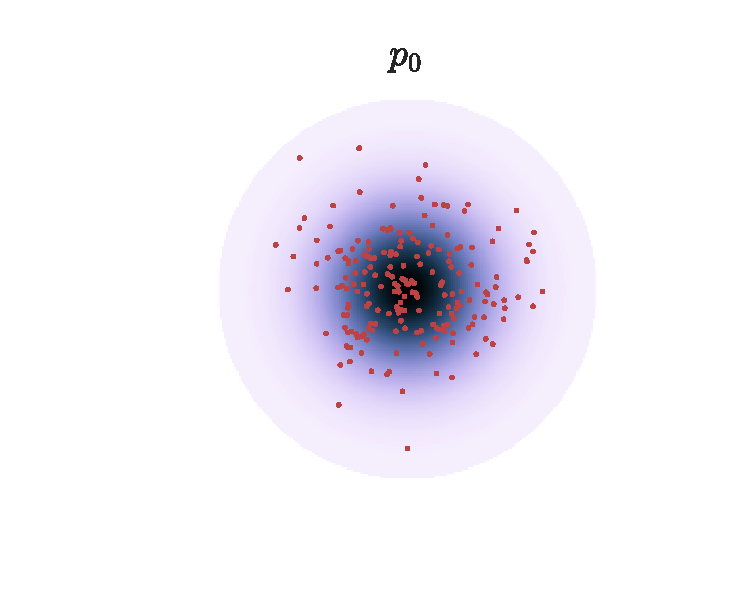
\includegraphics[scale=0.3,clip = true, trim=1cm 1.5cm 1cm 1.5cm]{figs/MEFN/normal_contours.pdf}&
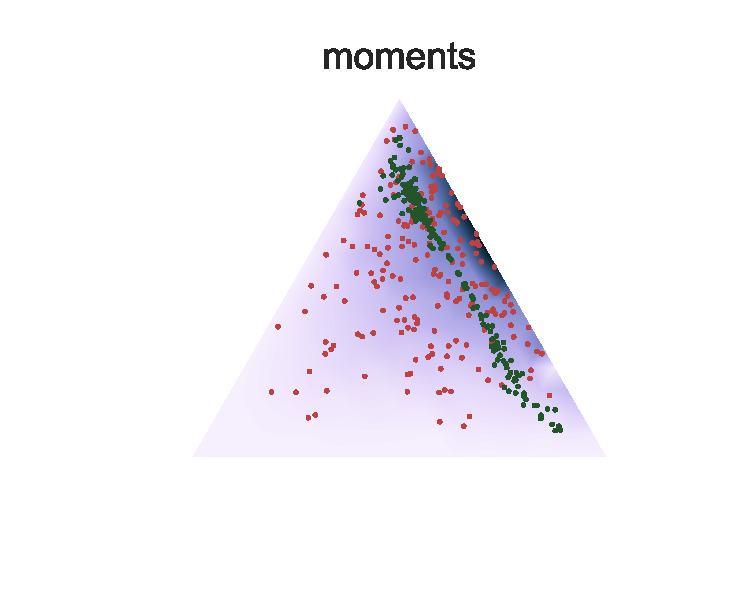
\includegraphics[scale=0.3,clip = true, trim=1cm 1.5cm 1cm 1.5cm]{figs/MEFN/network_contours_moments.pdf}&
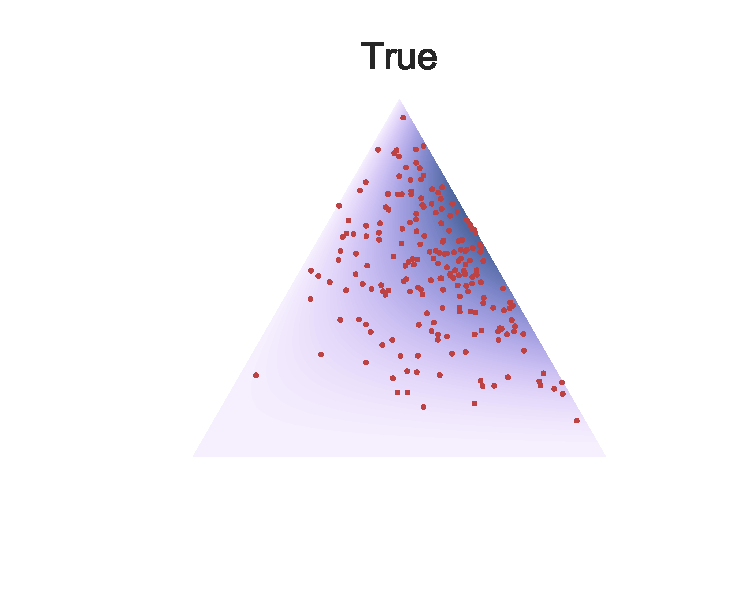
\includegraphics[scale=0.3,clip = true, trim=1cm 1.5cm 1cm 1.5cm]{figs/MEFN/true_contours.pdf}\\
{\scriptsize Initial distribution $p_0$}& \parbox{0.3\textwidth}{\scriptsize MEFN result $p_{\phi^*}$ (Control case: moment matching)}&{\scriptsize Ground truth $p^*$}\\
%& {\small (Control case: moment matching network)} & \\
%\\
\end{tabular}
\end{frame}

\begin{frame}
\frametitle{Experiment: Texture modeling}
\begin{itemize}
\item Sample from the space of images $\vz \in [0,1]^{224 \times 224 \times 3}$ where $T(\vz): [0,1]^{224 \times 224 \times 3} \rightarrow \mathbb{R}$ is a complicated ``texture loss'' defined in \cite{ulyanov2016texture}.
\item \cite{ulyanov2016texture} proposes texture net, which solves the problem by
\[\min E_{\mZ \sim p_0}\left[ T(f_\phi(\mZ)) \right] \]
without considering entropy term.
\item We compare our formulation with texture net. We use real-nvp \parencite{dinh2016density} as the normalizing flow structure
\end{itemize}
\end{frame}

\begin{frame}
\frametitle{Experiment: Texture modeling}
\centering
{\scriptsize
\begin{tabular}[t]{ccc}
Input & \hspace{-0.3cm} \parbox{0.3\textwidth}{\centering Texture net \\\parencite{ulyanov2016texture}} & \hspace{-0.3cm} MEFN (ours) \\
%\vspace{-0cm}
\includegraphics[scale=0.3,clip = true]{figs/MEFN/fig_texture_raw.jpg}&
\hspace{-0.3cm}\includegraphics[scale=0.3,clip = true]{figs/MEFN/fig_texture_noent_0.jpg}&
\hspace{-0.3cm}\includegraphics[scale=0.3,clip = true, trim=0cm 0cm 0cm 0cm]{figs/MEFN/fig_texture_ent_0.jpg}
\vspace{0.6cm}
\\
Texture cost & \hspace{-0.3cm} Negative entropy & \hspace{-0.3cm} RGB histogram\\
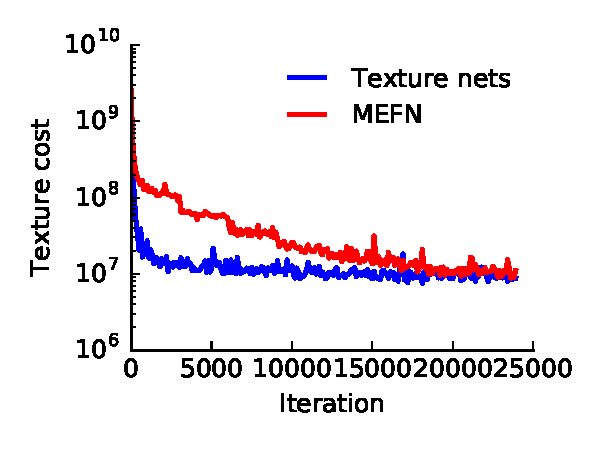
\includegraphics[scale=0.33,clip = true]{figs/MEFN/fig_texture_cost.pdf}&
\hspace{-0.3cm}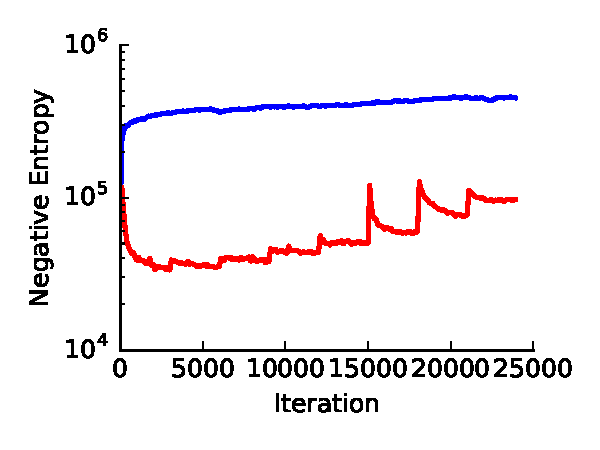
\includegraphics[scale=0.33,clip = true]{figs/MEFN/fig_texture_entropy.pdf}&
\hspace{-0.3cm}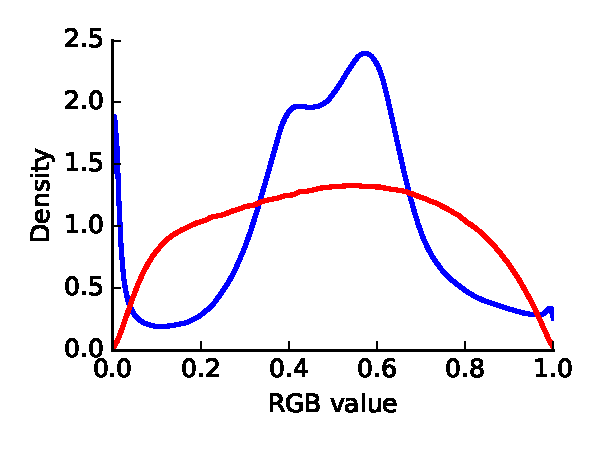
\includegraphics[scale=0.33,clip = true]{figs/MEFN/fig_texture_RGB_hist.pdf} \\
%\\
\end{tabular}
}
\end{frame}


\begin{frame}
\frametitle{Experiment: Texture modeling}
\begin{itemize}
\item We provide two numerical measure for assessing sample diversity given a set of images $\{\vz^{(1)},...,\vz^{(n)}\}$.
\end{itemize}
\centering
\begin{table}[htpb]
%\caption{Quantitative measure of image diversity using $20$ randomly sampled images}
%\label{sample-table}
\begin{center}
\begin{tabular}{l | l | lll}
Method  & $d_{L^2}$& SST & SSW & SSB \\
\hline 
Texture net  & 11534 & 128680 & 109577 & 19103\\
MEFN   & 17014 & 175604 & 161639 & 13964 \\
\end{tabular}
\end{center}
\begin{itemize}
\item Mean Euclidean distance: $d_{L^2} = \text{mean}_{i \neq j} \|\vz^{(i)} - \vz^{(j)} \|_2^2$
\item ANOVA: $\text{SST} = \text{SSW} + \text{SSB}$
\begin{itemize}
\item Total: $\text{SST} = \sum_{i,k} (z_k^{(i)} - \bar{z})^2$
\item Within group: $\text{SSW} = \sum_{i,k} (z_k^{(i)} - \bar{z}_k)^2$ (larger $\Rightarrow$ better)
\item Between group: $\text{SSB} = \sum_{k} n (\bar{z}_k - \bar{z})^2$ (smaller $\Rightarrow$ better)
\end{itemize}
\end{itemize}
\label{tab:texture}
\end{table}
\end{frame}

\begin{frame}
\frametitle{Conclusion and discussion}
\begin{itemize}
\item Summary
\begin{itemize}
\item Bridging information theory and deep learning
\item Solve maximum entropy problem by optimizing a normalizing flow
\item Combining augmented Lagrangian optimization with stochastic optimization
\item Promising result on simulation and real data
\end{itemize}
\item Future work
\begin{itemize}
\item Better normalizing flow structure
\item Better constrained stochastic optimization algorithm
\end{itemize}
\item Loaiza G*, \alert{Gao Y}*, Cunningham JP (2017) Maximum entropy flow networks. ICLR 2017. (*=equal contribution) 
\end{itemize}
\end{frame}

%\begin{frame}
%\frametitle{Acknowledgement}
%\end{frame}


\begin{frame}
\frametitle{Table of Contents}
\tableofcontents
\end{frame}

\begin{frame}
\frametitle{fLDS: AEVB form (backup)}
\end{frame}

\begin{frame}
\frametitle{MEFN: Normalizing flow structures (backup)}
\end{frame}

\end{document}


